% !TEX root = main.tex

\section{Introduction}

Symbolic execution is a very powerful static analysis technique. In this paper, we describe the main aspects of this methodology and discuss how symbolic execution has been extensively exploited in the context of computer security for analyzing code in both source and binary form.

\paragraph{Black-box approach versus white-box approach}

Discussion of black-box approach and white-box approach. Symbolic execution is a white-box technique. Black-box approaches can be very fast but not always effective. White-box approaches can be very effective but are typically slower than black-box techniques. An in-depth discussion of this aspect will be done when we will discuss~\cite{DRILLER-NDSS16}.

\begin{figure}[H]
  \vspace{-3mm}
  \centering
  \begin{subfigure}{.5\textwidth}
    \centering
    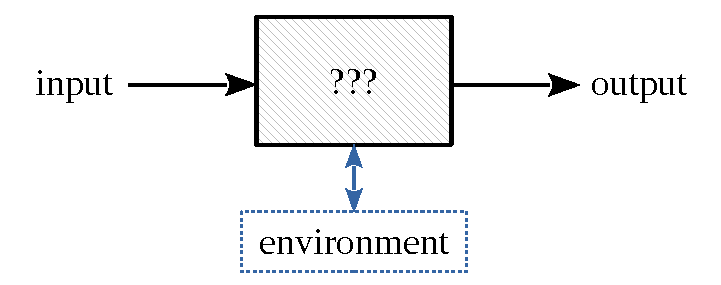
\includegraphics[width=0.9\linewidth]{images/blackbox} 
    \caption{Black-box approach}
    %\label{fig:sub1}
  \end{subfigure}%
  \begin{subfigure}{.5\textwidth}
    \centering
    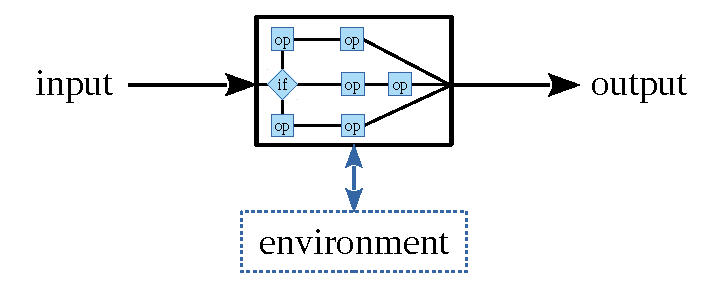
\includegraphics[width=0.9\linewidth]{images/whitebox} 
    \caption{White-box approach}
    %\label{fig:sub2}
  \end{subfigure}
  %\label{fig:example-symbolic-execution}
  \vspace{-3mm}
\end{figure}
